\chapter{\textit{Grasp}について}
\label{graspについて}

\section{概要}

\textit{grasp}は「把握」を意味する動詞・名詞だが、ここでの\textit{grasp}とは「人がある対象に注意や目的意識を抱き、注意を向けた対象を確かめるため、または目的の達成に向けて試行を行う期間」とする。手指の構造を変化させる本作は、このコンセプトに注目し、手指の構造の変換をきっかけに起こる注意や、変換した手指とボールとの関係のもとで生じる目的意識が、体験者の中で自発的に生まれることを目指した。本章では、この\textit{grasp}についての詳細を示す。\\

\section{\textit{grasp}の定義}
本研究での\textit{grasp}とは、「人がある対象に注意や目的意識を抱き、注意を向けた対象を確かめるため、または目的の達成に向けて試行を行う期間」であると定義する。
例えば、楽器の習得過程において、弾きこなしたいフレーズを定め、それを達成するまでに試行錯誤をし、達成できるようになるまでの期間を指す。また、そのように熟達していくと、熟達をきっかけとして別の目標が芽生える。当初目指していた、あるいはやってみる前から想起できていたこととは異なることについて目的意識が芽生える。\\
これは\textit{grasp}の過程における重要な性質の1つであると考えている。

\section{Felsの議論との関係性}
このコンセプトについて、FelsのEmbodimentのカテゴリ、並びにIntimacyとの関係性を明確にする。\\

\section{\textit{grasp}の性質}
\textit{grasp}には二つの性質がある。一つは、時間幅が注意を向けている対象によって、長い場合と短い場合があることである。目的意識が芽生えてからスムーズに操作できるようになる場合、'reach'から'manipulate'が近く、\textit{grasp}は短い、すなわち直感的で使いやすいものとして経験される。その一方、目的意識が芽生えてから試行錯誤を伴い、習熟に長い期間を要する場合、\textit{grasp}は長く、もどかしさを経験し、操れるようになった時に達成感を経験する。\\

二つ目に、\textit{grasp}の過程で他のことに対する意識が次々と芽生えることがある。具体的には「やってみるまでわからない」といった経験や、物事に対する解像度が高まる中で、当初とは異なる意識が芽生える状況に相当する。\\

このコンセプトを展開し、「試行錯誤の余地」を設計することを目指したのが、修士作品「Grasp(er)」である。この作品では、\textit{grasp}を経験する中で、個人による創造的な活動が生まれ、\textit{grasp}という動作を行っているのではなく、そこに'er'の接尾辞がついた'Grasper'であると名付けた。

'Grasper'は、「Familiar / Strange」と「Relation」という二つから構成された作品群である。これらに共通する目的は、\textit{grasp}の中で個人が目的意識や興味を抱くことで、\textit{grasp}が連鎖的に生じることである。制作者は「このようなことをしてほしい」という行為の中身を設計せず、体験する個人がその中で次々と注目する対象を見出すことによって、個人が行為を創造していくことを目指している。

このため、「手指の構造や、手指を取り巻く環境を変化させることで、手指の運動に注目する構造」を作ることに取り組んだ。このときの「注目」が起点となって\textit{grasp}の期間が生じるが、その先々で起こる体験は個人に委ねられ、明示的な目的は設定されていない。

この作品群の筐体の設計は、画面の中に出力される図像が「自分の手指に替わる存在」として認識されるように意図されている。体験中に意識が集中できるような構成が目指され、手指を動かす際にはできるだけ自由に動かせるようになっている。

\section{「Grasp(er)」におけるコンセプトの適用}
本作品の作品構造については次章で詳しく述べるが、ここではこのコンセプトが修士作品「Grasp(er)」においてどのように適用されているかについて説明する。\\
\subsection{基本構造}
「身体の変容」を扱っている本作では、取得されたキーポイントの位置を大きく変更させることで、「意図的にIntimacyを下げる」操作を行なっている。しかし「下がった」という事実を体験者が認識するために、もとの手が鏡合わせのように出力されている状態から、徐々に形を変えていくようすを連続的に示すモーフィングを実装している。\\
過去に展示していたバージョンではモーフィングを示さず、手指が認識されたとたんに全く違う手指が提示される作品形態であった。しかし、この形態で展示した場合、画面の中の手指と自身の関係性について、全く異なる生命体のようなものを、操り人形のように自分の手指の指令によって動かす、といったような関係性として認識されることがあった。また、全く見慣れない形なので、「手指を細かく動かせる」といった、作品がもつ可能性に気づけない場合があることがわかった。そこで、このモーフィングを実装することで、白い点が関節を表していること、そして手指の運動を細かくトラッキングしていることを事前に伝え、それが形を変えた姿として画面の前に提示されていることを示す形態を採用することになった。
そうすることで、画面に出力されているグラフィックと身体との関係性は別々の存在ではなく、自分の身体であったことが明示される。\\
\subsection{Familiar / Strange}
この作品は、3分10秒で1ループの構造になっている。それぞれの変換は、線形補完やゴム紐が切れた時のような振動を伴う動きによって補完される。シーン遷移を説明する図を以下に示す。
\begin{figure}[H]
  \centering
  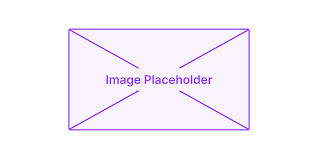
\includegraphics[width=15cm]{img/placeholder.png}
  \caption{Familiar / Strange}
  \label{fig:diagram_familiar_strange}
\end{figure}

\subsection{Relation}